\documentclass[tikz,convert={outfile=\jobname.svg}]{standalone}
\usepackage[arrowmos]{circuitikz}
\begin{document}
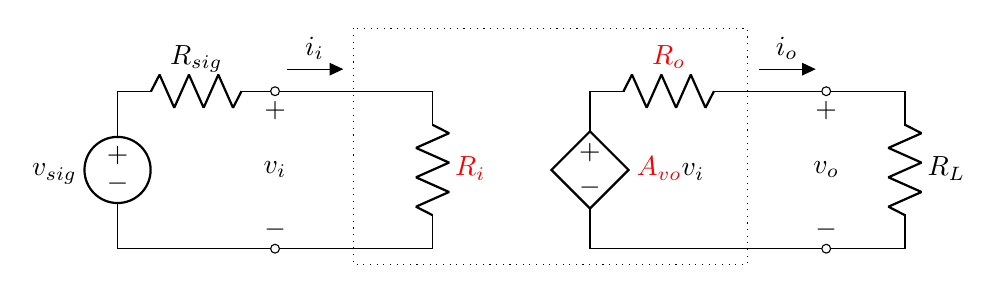
\begin{tikzpicture}
  \draw
  (0, 0)
  to[american voltage source, l_=$v_{sig}$] ++(0, -2)
  to[short, -o] ++(2, 0) node[above] {$-$}
  -- ++(2, 0)
  to[R, l_=$\textcolor{red}{R_i}$] ++(0, 2)
  -- ++(-1, 0)
  to[short, f_<=$i_i$] ++(-1, 0) node[below] {$+$}
  to[R, l_=$R_{sig}$, o-] ++(-2, 0)
  ++(2, -1) node[] {$v_i$}

  (6, 0)
  to[american controlled voltage source, l=$\textcolor{red}{A_{vo}}v_i$] ++(0, -2)
  to[short, -o] ++(3, 0) node[above] {$-$}
  -- ++(1, 0)
  to[R, l_=$R_L$] ++(0, 2)
  -- ++(-1, 0) node[below] {$+$}
  to[short, f<_=$i_o$, o-] ++(-1, 0)
  to[R, l_=$\textcolor{red}{R_o}$] ++(-2, 0)
  ++(3, -1) node[] {$v_o$}
  ;
  \draw[dotted] (3, 0.8) rectangle (8, -2.2);
\end{tikzpicture}
\end{document}
